\documentclass[12pt,oneside]{memoir}

% \usepackage[utf8]{inputenc}
\usepackage{cmsrb}
\usepackage{listings}
\usepackage{matfmaster}
\usepackage{url}
\usepackage{graphicx}
\usepackage{float}
\usepackage{hyperref}

\usepackage{color}
\definecolor{lightgray}{rgb}{.9,.9,.9}
\definecolor{darkgray}{rgb}{.4,.4,.4}
\definecolor{purple}{rgb}{0.65, 0.12, 0.82}
\definecolor{customGreen}{rgb}{0.25, 0.85, 0.25}

\lstdefinelanguage{Swift}{
  keywords={associatedtype, class, deinit, enum, extension, fileprivate, func, import, init, inout, internal, let, open, operator, private, precedencegroup, protocol, public, rethrows, static, struct, subscript, typealias, var, break, case, catch, continue, default, defer, do, else, fallthrough, for, guard, if, in, by, repeat, return, throw, switch, where, while, Any, as, catch, false, is, nil, rethrows, self, Self, super, throw, throws, true, try, _, associativity, convenience, didSet, dynamic, final, get, indirect, infix, lazy, left, mutating, none, nonmutating, optional, override, postfix, precedence, prefix, Protocol, required, right, set, some, Type, unowned, weak, willSet, @State, List, View, Image, VStack, Text, color, action},
  keywordstyle=\color{blue}\bfseries,
  ndkeywords={Int, String, Double, Float, Bool},
  ndkeywordstyle=\color{customGreen}\bfseries,
  identifierstyle=\color{black},
  sensitive=false,
  comment=[l]{//},
  morecomment=[s]{/*}{*/},
  commentstyle=\color{purple}\ttfamily,
  stringstyle=\color{orange}\ttfamily,
  morestring=[b]',
  morestring=[b]"
}

\lstset{
   language=Swift,
%   backgroundcolor=\color{datgray},
   extendedchars=true,
   basicstyle=\footnotesize\ttfamily,
   showstringspaces=false,
   showspaces=false,
   numbers=left,
   numberstyle=\footnotesize,
   numbersep=9pt,
   tabsize=4,
   breaklines=true,
   showtabs=false,
   captionpos=b
}

\bib{literatura}

\autor{Марко Вељковић}
\naslov{Креирање виџета у програмском језику Swift}
\godina{2022}
\mentor{др Милена \textsc{Вујошевић Јаничић}, ванредни професор\\ Универзитет у Београду, Математички факултет}
\komisijaA{др Филип \textsc{Марић}, ванредни професор\\ Универзитет у Београду, Математички факултет}
\komisijaB{др Мирко \textsc{Спасић}, доцент\\ Универзитет у Београду, Математички факултет}
\datumodbrane{15. јануар 2022.}

\apstr{
Употреба програмског језика \textit{Swift} за израду виџета у \textit{iOS} оперативном систему
}

\kljucnereci{\textit{widget},  \textit{Swift}, \textit{iOS}, \textit{Apple}, програмски језик, програмирање}

\begin{document}

\frontmatter
\naslovna
\komisija
\apstrakt
\tableofcontents*

\mainmatter

\chapter{Увод}

\chapter{Програмски језик Swift}

\indent \textit{Swift} је модеран програмски језик, првенствено намењен развоју  апликациjа на \textit{Apple} платформама (\textit{iOS}, \textit{iPadOS}, \textit{macOS}, \textit{tvOS} и \textit{watchOS}). Настао је као резултат истоименог пројекта унутар компаније \textit{Apple}, чији је циљ био креирање програмског језика  који ће бити сигуран, концизан и ефикасан. Резултати пројекта \textit{Swift} биће приказани у наставку. 

\section{Настанак и развој}

\indent Развој програмског језика \textit{Swift} започео је Крис Латнер (енг. Chris Lattner) \footnote{Софтверски инжењер, најпознатији по развоју \textit{LLVM}  технологија, \textit{Clang} компајлера и \textit{Swift} програмског језика} у јулу 2010. године. У јуну 2014. године објављена је прва апликација комплетно написана у \textit{Swift}-у, названа "Apple Worldwide Developers Conference" (WWDC) по истоименој годишњој конференцији информационих технологија компаније \textit{Apple}. На конференцији те године, кроз предавање и интерактивну демонстрацију представљена је бета верзија језика, "The Swift Programming Language" \cite{The_Swift_Programming_Language} - бесплатно упутство и званична веб страница \cite{SwiftOfficialSite}. Прва званична верзија језика \textit{Swift} 1.0, постала је доступна 9. септембра 2014. године.

\indent Званично објављивање апликација (на \textit{App Storе}-у) писаних у \textit{Swift}-у постало је могуће од верзије програмског језика 2.0. Језик је у оквиру анкете коју организује  \textit{Stack Overflow}  \cite{StackOverflow} проглашен за омиљени програмски језик 2015. године, док је 2016. године заузео друго место у тој категорији. Децембра 2015. изворни код језика, подржаних библиотека, дибагер и менаџер пакета постали су отвореног кода, под лиценцом \textit{Apache} 2.0, доступни на \textit{GitHub}-у \cite{GitHub_Swift}.

\indent На годишњој конференцији 2016. године представљена је апликација за уређај \textit{iPad} под називом \textit{Swift Playgrounds} \cite{Swift_Playground}, која је намењена учењу програмирања у \textit{Swift}-у. Касније је ова апликација развијена и за оперативни систем \textit{macOS}.

\indent Током конференције 2019. године представљено је радно окружење \textit{SwiftUI} \cite{Swift_SwiftUI}, које омогућава декларативно програмирање апликација за све \textit{Apple} платформе. У време писања рада, последња званична верзија језика је \textit{Swift} 5.6.

\section{Основна намена и карактеристике}

\begin{figure}[H]

\includegraphics[width=0.5\textwidth]{images/Swift_logo.png}
\centering
\caption{\textit{Swift лого}}
\label{slika:swift_logo}
\end{figure}

\indent \textit{Swift} је моћан и интуитиван језик за програмирање апликација намењних \textit{Apple} платформама (\textit{iOS}, \textit{iPadOS}, \textit{macOS}, \textit{tvOS} и  \textit{watchOS}). Писање кода у \textit{Swift}-у је забавно и лако, синтакса је веома концизна, али у исто време веома изражајна. Програмски језик \textit{Swift} је безбедан, брз и интерактиван, и као такав погодан за људе који уче основе програмирања. Код писан у \textit{Swift}-у се преводи и оптимизује тако да извуче максимум из хардверских компоненти. 
Детаљнији опис особина и примери кодирања биће дати у наредним одељцима. 

\section{Концепти}
\label{sec:Концепти}

\indent \textit{Swift} је наследник програмских језика \textit{C} и \textit{Obјective-C}, па је самим тим одређенe концепатe преузео из ових језика, али истовремено постоје концепти у \textit{Swift}-у који нису присутни у \textit{C}-у и \textit{Obјective-C}-у. Објашњење најбитнијих концепата у \textit{Swift}-у дат је у наставку, док се потпуна листа може наћи на званичком сајту програмског језика. \cite{SwiftOfficialSite}

\subsection{Основе}

\indent \textit{Swift} пружа своје типове основних променљивих, \textit{Int} за целобројне вредности, \textit{Float} и \textit{Double} за бројеве са основом у покретном зарезу, \textit{Bool} за Булове вредности, \textit{String} за текстуалне променљиве, као и три основна типа колекција \textit{Array}, \textit{Set} и \textit{Dictionary} о којима ће бити више речи у делу \ref{subsec:Колекције} \nameref{subsec:Колекције}. 
\\ 
\indent Поред ових основних типова који су наслеђени из \textit{Objective-C}-а, постоје и неколико ново уведених, као што су \textit{Tuples} који омогућују креирање и прослеђивање груписаних вредности и \textit{Optionals} помоћу којих рукујемо \textit{nil} вредношћу на безбедан начин.
\\
\indent Константе декларишемо коришћењем кључне речи \textit{let}, након чега следи име константе и затим њена иницијализација. Декларисање променљиве постижемо употребом кључне речи \textit{var}. Када декларишемо променљиво можемо је одмах и иницијализовати или коришћењем анотације јој само доделити тип. Конкретна примена се може видети у примеру \ref{lst:Декларисања променљивих и константи} - \nameref{lst:Декларисања променљивих и константи}.

\begin{lstlisting}[caption=\textit{{Декларисања променљивих и константи}}, label={lst:Декларисања променљивих и константи}, language=Swift, frame=single]
// Deklarisanje konstantne
let spageteKarbonaraRecept = Recept("Spagete Karbonara")

// Deklarisanje promenljive uz inicijalizaciju
var raspolozivoNovca = 1000

// Deklarisanje promenljive koriscenjem samo anotacije
var brojPorcija: Int
\end{lstlisting}

\indent Целобројне променљиве могу бити написане у облику децималних, бинарних, окталних и хексадецималних бројева. Пример следи у наставку \ref{lst:Целобројне променљиве} - \nameref{lst:Целобројне променљиве}.

\begin{lstlisting}[caption=\textit{{Целобројне променљиве}}, label={lst:Целобројне променљиве}, language=Swift, frame=single]
let mojiBroj = 25 
let binarniBroj = 0b11001     // 25 u binarnom obliku
let oktalniBroj = 0o31        // 25 u oktalnom obliku
let heksadecimalniBroj = 0x19 // 25 u heksadecimalnom obliku
\end{lstlisting}

\indent \textit{Tuple} група се користи за груписање променљивих било ког типа. Група може садржати променљиве различитих типова. У примеру \ref{lst:Tuple} - \nameref{lst:Tuple}, могу се видети два начина креирања \textit{Tuple} група и различити начини приступања члановима групе.

\begin{lstlisting}[caption=\textit{{Tuple}}, label={lst:Tuple}, language=Swift, frame=single]
// Definisanje tuple-a (String, Int)
let namirnicaSaCenom = ("Jaja 10 komada", 100)

// Pristupanje clanovima tuple-a:
let namirnica = namirnicaSaCenom.0
let cena = namirnicaSaCenom.1

// Definisanje tuple-a sa imenovanim clanovima
let urednijaNamirnicaSaCenom = (namirnica: "Jaja 10 komada", cena: 100)

// Pristupanje imenovanim clanovima tuple-a::
let urednijaNamirnica = urednijaNamirnicaSaCenom.namirnica
let urednijaCena = urednijaNamirnicaSaCenom.cena
\end{lstlisting}

\indent \textit{Assertions} %TODO

\subsection{Оператори}

\indent Као и у већини програмских језика, постоје три основне врсте оператора: 

\begin{itemize}
  \item Унарни
  
\begin{itemize}
    \item Префиксни унарни оператори (на пример, '-' за бројевне вредности и '!' за логичке вредности)  
    \item Постфиксни унарни оператори (на пример, '?' и '!' који се користе за опционе променљиве)
\end{itemize}
  
  \item Бинарни 
  
\begin{itemize}
    \item Оператор доделе '=', који за разлику од језика C, не враћа повратну вредност  
    \item Артиметички оператори, '+', '-', '*', '/', '\%'
    \item Сложени оператори доделе, '+=', '-=', '*=', '/='
    \item Оператори поређења, '==', '!=', '<', '>', '<=', '>='
\end{itemize}
 
  \item Тернарни \\
  Једини тернари оператор који постоји у језику је оператор '?:'. Код овог оператора израз са крајње леве стране мора бити типа \textit{Bool}, док израз или променљива која се налази у средини оператора мора бити истог типа као израз или променљива са крајње десне стране, без ограничења типа. Пример примене тернарног оператора, као и приказ блока кода који једна линија са тернарним оператором може заменити приказани су у примеру \ref{lst:Тернарни оператор} - \nameref{lst:Тернарни оператор}.
  
\begin{lstlisting}[caption=\textit{{Тернарни оператор}}, label={lst:Тернарни оператор}, language=Swift, frame=single]
// Ternarni operator:
a ? b : c

// Izraz ternarnog operatora 
let visinaCelije = celijaImaSliku ? 100 : 50

// Prethodni primer koriscenjem uslovnog grananja
let visinaCelije: Int
if celijaImaSliku {
    visinaCelije = 100
}
else {
    visinaCelije = 50
}
\end{lstlisting}
\end{itemize}

\indent Поред основних оператора у \textit{Swift}-у постоје и специјалне врсте оператора

\begin{itemize}
    \item Оператор 'nil-сједињавања' ('??'), бинарни оператор који се користи над опционим променљивима. Уколико израз са леве стране оператора садржи вредност (није \textit{nil}), та вредност ће бити резултат оператора, док уколико је лева страна оператора једнака  \textit{nil}, резултат оператора биће израз са десне стране, који мора садржати неку вредност. Пример примене '??' оператора и приказ његовог расписивања помоћу тернарног оператора дат је у наставку \ref{lst:nil-сједињавање} - \nameref{lst:nil-сједињавање}.
    
    \begin{lstlisting}[caption=\textit{{nil-сједињавање}}, label={lst:nil-сједињавање}, language=Swift, frame=single]
    var a: Int?
    if trenutnoVremeUMilisekundama % 2 == 0 {
        a = 10
    }
    // Ukoliko promenljiva 'a' ne sadrzi vrednost, promenljivoj 'b' bice dodeljena vrednost 5
    let b = a ?? 5
    
    // Raspisivanje operator 'nil-sjedinjavanja' koriscenjem ternarnog operatora:
    let b = (a != nil ? a! : 5)
    \end{lstlisting}
    
    \item Оператори распона
    
\begin{itemize}
    \item Затвореног распона (а...b), распон од 'а' до 'б' укључујући оба броја
    \item Полу-отвореног распона (а..<b), распон од 'а' до 'б' укључујући само 'а'
    \item Распони једне стране [a...], распон од 'а' па надаље докле год је то могуће (Ову врсту оператора треба користити опрезно!)
\end{itemize}

\end{itemize}

\subsection{Карактери и стрингови}

\indent Стринг је низ карактера, као што је "Здраво, свете". У \textit{Swift}-у се стрингови представљају помоћу класе \textit{String}, која омогућава брз, ефикасан и \textit{Unicode}-компатибилан начин рада са текстом. Креирање и операције са стринговима (конкатенација, рад са карактерима и интерполација) биће приказане кроз пример \ref{lst:Операције над стринговима} - \nameref{lst:Операције над стринговима}.

\begin{lstlisting}[caption=\textit{{Операције над стринговима}}, label={lst:Операције над стринговима}, language=Swift, frame=single]
    var prazanString = ""
    var drugiPrazanString = String()
    var treciPrazanString: String?
    
    if !prazanString.isEmpty {
        prazanString = "Zdravo"
    }
    
    // Konkatenacija stringova
    drugiPrazanString += ", svete"
    
    // Rad sa karakterima
    for k in prazanString {
        print(k)
    }
    // Ispisace: 
    // Z
    // d
    // r
    // a
    // v
    // o
    
    // Interpolacija stringova
    print(\(prazanString) + \(drugiPrazanString) + "!")
    // Ispisace 'Zdravo, svete!'
\end{lstlisting}


\subsection{Колекције}
\label{subsec:Колекције}

\indent \textit{Swift} дефинише три примарна типа колекција: низове, скупове и речнике. Сва три типа су дефинисана као генеричке\footnote{Генерички код омогућава писање флексибилних и поновно искористивих функција и типова; помоћу њих се избегава непотребно дуплирање кода} колекције. Уколико се дефинисана колекција додели променљивој, она се може мењати (додавање, брисање и измена чланова у њој); међутим уколико се она додели некој константи, манипулација њеним члановима неће бити могућа. \\

\indent Низови се користе за уређено чување елемената истог типа. Један елемент се може појавити у низу више пута, на различитим индексима. Конкретан пример дефинисања, иницијализације и управљањем података низа може се видети у коду \ref{lst:Рад са низовима} - \nameref{lst:Рад са низовима}.

\begin{lstlisting}[caption=\textit{{Рад са низовима}}, label={lst:Рад са низовима}, language=Swift, frame=single]
    // Definisanje niza sa elementima tipa 'Recept'
    var recepti: [Recept] = []
    // Dodavanje novog elementa
    recepti.append(Recept("Domaca kafa"))
    // Pristupanje prvom clanu niza
    var prviRecept = recepti[0]
    // Kreiranje niza sa 3 inicijalna elementa tipa 'String'
    var koraci = Array(repeating: "", count: 3)
    // Foreach petlja kojom prolazimo kroz niz uz pamcenje indeksa
    for (index, korak) in prviRecept.koraci.enumerated() {
        if index < 3 {
            koraci[index] = korak
        }
        else {
            koraci.append(korak)
        }
    }
    // Brisanje prvog clana niza, ukoliko niz nije prazan
    if !koraci.isEmpty {
        koraci.remove(at: 0)
    }
\end{lstlisting}

\indent Скупови су колекције које не гарантују чување редоследа елемената и у којима један елемент може да се појави највише једанпут. Тип елемента скупа мора бити могуће кодирати\footnote{Тип који се може кодирати мора имати дефинисану функцију за одређивање hash вредности за сваку инстанцу, два елемента могу имати исту hash вредност акко су једнаки} (енг. hashable). Рад са скуповима приказан је у примеру \ref{lst:Рад са скуповима} - \nameref{lst:Рад са скуповима}.

\begin{lstlisting}[caption=\textit{{Рад са скуповима}}, label={lst:Рад са скуповима}, language=Swift, frame=single]
    // Kreiranje skupa sa elementima tipa 'String'
    var sastojci = Set<String>()
    // Dodavanje novog elementa
    sastojci.insert("Mlevena kafa")
    
    // Provera broja elemenata skupa
    if sastojci.count == 1 {
        sastojci.insert("Obicna voda")
    }
    
    // Provera da li odredjeni element postoji u skupu
    if sastojci.contains("Secer") {
        sastojci.remove("Secer")
    }
    else {
        sastojci.insert("Mleko")
    }
    
    var dodatniSastojci = Set<String>()
    dodatniSastojci.insert("Mleko")
    
    // Rad sa skupovnim operacijama
    
    // Unija
    sastojci.union(dodatniSastojci)
    // Mlevena kafa, Obicna voda, Mleko
    
    // Presek
    sastojci.intersection(dodatniSastojci)
    // Mleko
    
    // Razlika
    sastojci.subtracting(dodatniSastojci)
    // Mlevena kafa, Obicna voda
    
    // Disjunktivna unija
    sastojci.symmetricDifference(dodatniSastojci)
    // Mlevena kafa, Obicna voda
\end{lstlisting}

\indent Речници се користи за чување скупа парова кључ - вредност, без очувања редоследа. Свака вредност је додељена јединственом кључу, који мора бити погодан за кодирање (енг. hashable). Речници се најчешће користе за чување података којима је могућ брз приступ помоћу одговарајућег кључа. Рад са речницима приказан је у прмеру \ref{lst:Рад са речницима} - \nameref{lst:Рад са речницима}.

\begin{lstlisting}[caption=\textit{{Рад са речницима}}, label={lst:Рад са речницима}, language=Swift, frame=single]
    // Kreiranje recnika tipa [Int : String]
    var tipoviHTTPStatusa: [Int : String] = [:]
    
    // Dodeljivanje recnika promenljivoj 'tipoviHTTPStatusa'
    tipoviHTTPStatusa = [200: "OK", 201: "Resurs je kreiran", 202: "Zahtev je prihvacen"]
    
    // Dodavanje novog elementa ukoliko ne postoji, odnosno promena postojeceg
    tipoviHTTPStatusa[404] = "Stranica nije pronadjena"
    
    // Brisanje elementa iz recnika
    if let izbrisanaVrednost = tipoviHTTPStatusa.removeValue(forKey: 201) {
        print("Vrednost izbrisana iz recnika: \(izbrisanaVrednost)")
    }
    
    // Razlicite vrste iteracija kroz recnik
    
    for kod in tipoviHTTPStatusa.keys {
        // TODO: iteriraj kroz kodove
    }
    
    for status in tipoviHTTPStatusa.values {
        // TODO: iteriraj kroz statuse
    }

    for (kod, status) in tipoviHTTPStatusa {
        // TODO: iteriraj kroz elemente
    }
\end{lstlisting}

\subsection{Контрола тока}

\indent Наредбе контроле тока које се користе у \textit{Swift}-у су: \textit{if}, \textit{guard}, \textit{switch} и петље: \textit{for-in}, \textit{while}. \textit{If} наредба приказана је у примеру \ref{lst:If наредба контроле тока} - \nameref{lst:If наредба контроле тока}.

\begin{lstlisting}[caption=\textit{{If наредбa контроле тока}}, label={lst:If наредба контроле тока}, language=Swift, frame=single]
    var recept = Recept("Cezar salata")
    recept.sastojci = ["Zelena salata", "Pilece grudi", "Slanina", "Paradajz", "Hleb", "Cezar premaz"]
    // If naredba kondtrole toka
    var brojSastojaka = recept.sastojci.count
    if brojSastojaka < 6 {
        print("Neki sastojak nedostaje")
    }
    else if brojSastojaka > 6 {
        print("Broj sastojaka ne odgovara originalu, ali samo napred, eksperimentisi")
    }
    else {
        print("Broj sastojaka je odgovarajuci")
    }
\end{lstlisting}

\indent \textit{Switch} наредба је слична као у другим програмским језицима, једна битна разлика је да ће се увек извршити тачно један од случајева унутар наредбе, па није потребно експлицитно навођење \textit{break} наредбе. \textit{Break} наредба се по конвенцији наводи само када је неки од случајева \textit{Switch} наредбе празан, јер сваки случај мора бити извршив (енг. executable). Наведене ствари приказане су у примеру \ref{lst:Switch наредба контроле тока} - \nameref{lst:Switch наредба контроле тока}.

\begin{lstlisting}[caption=\textit{{Switch наредба контроле тока}}, label={lst:Switch наредба контроле тока}, language=Swift, frame=single]
    enum Zacin {
        case vegeta, kari, kurkuma, origano, biber
    }
    
    var mojiZacin: Zacin = .vegeta
    
    // Switch naredba
    switch mojiZacin {
        case .vegeta:
            print("Vegeta")
        case .biber:
            print("Nije vegeta, nego biber")
        default:
            print("Nije vegeta ni biber")
    }
    
    // Ukoliko ne navedemo sve slucajeve, moramo dodati slucaj 'default' slucaj
    switch mojiZacin {
        case .origano:
            print("Moze i to")
        default:
            break
    }
\end{lstlisting}

\indent \textit{For-in} је наредба понављања која се користи за пролаз кроз елементе неке колекције (низа, скупа, речника). Променљива која се користи за пролаз кроз колекцију је увек константа и није је могуће мењати у телу наредбе. Један од начина на који можемо мењати елементе колекције (уколико је колекција дефинисана као променљива, коришћењем кључне речи \textit{var}) је истовременим пролажењем кроз елементе и њихове индексе колекције и променом елемента колекције на одређеној позицији. Описани начине употребе петље могу се видети у примеру \ref{lst:For-in наредба контроле тока} - \nameref{lst:For-in наредба контроле тока}.
\begin{lstlisting}[caption=\textit{{For-in наредбa контроле тока}}, label={lst:For-in наредба контроле тока}, language=Swift, frame=single]
    let sastojci = ["Jaja", "Pecenica", "Maslinovo ulje", "Persun"]
    // For-in naredba
    for sastojak in sastojci {
        print("Potreban sastojak: \(sastojak)")
    }
    
    let sastojciSaKolicinom = ["Jaja": "3 komada", "Pecenica": "50 grama", "Maslinovo ulje": "Koliko je potrebno da pokrije tiganj", "Persun": "Prstohvat"]
    // For-in naredba za prolaz kroz recnik
    for (sastojak, kolicina) in sastojciSaKolicinom {
        print("Potreban sastojak: \(sastojak), u kolicini: \(kolicina)")
    }
    
    var promenljiviElementi = ["Jaja", "Pecenica", "Maslinovo ulje", "Persun"]
    // For-in naredba sa indeksiranjem
    for (indeks, element) in promenljiviElementi.enumerated() {
        if element == "Persun" {
            promenljiviElementi[indeks] = "Origano"
        }
    } 
\end{lstlisting}

\indent Постоје два типа \textit{while} наредбе понављања. \textit{While} наредба која прво проверава да ли је задати услов испуњен и онда извршава тело петље и \textit{repeat-while} наредба која прво извршава тело наредбе након чега проверава услов и уколико је он задовољен наставља са следећом итерацијом. Употреба је приказана у примеру \ref{lst:While наредба контроле тока} - \nameref{lst:While наредба контроле тока}. 

\begin{lstlisting}[caption=\textit{{While наредбa контроле тока}}, label={lst:While наредба контроле тока}, language=Swift, frame=single]
    let nasumicniBrojevi = [3, 12, 5, 18, 11, 99]
    var i = 0
    // While naredba
    while i < nasumicniBrojevi.count, nasumicniBrojevi[i] < 15 {
        print("Broj \(nasumicniBrojevi[i] je manji od 15")
        i += 1
    }
    
    let nasumicniBroj = nasumicniBrojevi[2] // 5
    // Repeat-while petlja
    repeat {
        print("Zdravo, svete!")
    } while nasumicniBroj != 5 // Uvek netacno
\end{lstlisting}

\begin{lstlisting}[caption=\textit{{Додаци наредбa контроле тока}}, label={lst:Додаци наредба контроле тока}, language=Swift, frame=single]
    //TODO: continue, break, fallthrough, return, throw
\end{lstlisting}

\subsection{Функције и затворења}

\indent Фунцкије су делови кода, који обично имају само једну, специфичну намену. Свака функција је идентификована својим именом које се користи да би се конкретна функција позивала у коду. Поред имена, функција може имати повратну вредност (уколико није дефинисана, подразумевана повратна вредност је \textit{Void}) и пареметре (именоване или неименоване). %TODO: prepraviti primere

\begin{lstlisting}[caption=\textit{{Дефинисање и позивање функције са параметром}}, label={lst:Дефинисање и позивање функције са параметром}, language=Swift, frame=single]
    // Definisanje fukncije
    func ispisiSastojke(sastojci: [String]) {
        for sastojak in sastojci {
            print(sastojak)
        }
    }
    
    let sastojci = ["Jaja", "Sira"]
    // Pozivanje f-je 'ispisiSastojke'
    ispisiSastojke(sastojci: sastojci)
\end{lstlisting}

\begin{lstlisting}[caption=\textit{{Дефинисање и позивање функције са повратном вредношћу}}, label={lst:Дефинисање и позивање функције са повратном вредношћу}, language=Swift, frame=single]    
    // Definisanje funkcije koja ima povratnu vrednost 'Int' i jedan neimenovani parametar
    func izracunajCenu(_ proizvodi[String: Int]) -> Int {
        int ukupnno = 0
        for (proizvod, cena) in proizvodi {
            ukupno += cena
        }
        return ukupno
    }
    
    let proizvodi = ["Jaja": 10, "Sira": 200]
    // Kada f-ja ima neimenovane parametre, njihova imena(labele) ne navodimo prilikom pozivanja te funkcije
    let ukupnaCena = izracunajCenu(proizvodi)
\end{lstlisting}
    
\begin{lstlisting}[caption=\textit{{Дефинисање и позивање функције са параметрима са подразумеваним вредностима}}, label={lst:Дефинисање и позивање функције са параметрима са подразумеваним вредностима}, language=Swift, frame=single]
    // Definisanje fukncije koja nema povratnu vrednost, jedan imenovani parametar i jedan imenovani parametar (cija se labela razlikuje od imena promenljive) sa podrazumevanom vrednoscu
    func func ispisiSastojkeSaDvaparametra(sastojci: [String], ispisati ispisatiCeloIme: Bool = true) {
        for sastojak in sastojci {
            if ispisatiCeloIme {
                print(sastojak)
            }
            else {
                print(sastojak.prefix(3))
            }
        }
    }
    
    // Iskoristicemo primer niza sastojaka kao za f-ju 'ispisiSastojke'
    // Pozivanje f-je 'ispisiSastojkeSaDvaparametra' prosledjivanjem oba paremetra
    // Ovde mozemo videti da se prilikom poziva f-je, ukoliko je neki parametar imenovan, navodi njegova labela
    ispisiSastojkeSaDvaparametra(sastojci: sastojci, ispisati: false)
    ispisiSastojkeSaDvaparametra(sastojci: sastojci, ispisati: true)
    
    // Ukoliko ne navedemo drugi parametar 'ispisati', on ce u f-ji imati podrazumevanu vrednost, u ovom slucaju 'true'
    ispisiSastojkeSaDvaparametra(sastojci: sastojci)
\end{lstlisting}
\begin{lstlisting}[caption=\textit{{Дефинисање и позивање функције са повратном вредношћу}}, label={lst:Дефинисање и позивање функције са повратном вредношћу}, language=Swift, frame=single]    
    // Definisanje funkcije koja ima povratnu vrednost 'Int' i jedan neimenovani parametar
    func izracunajCenu(_ proizvodi[String: Int]) -> Int {
        int ukupnno = 0
        for (proizvod, cena) in proizvodi {
            ukupno += cena
        }
        return ukupno
    }
    
    let proizvodi = ["Jaja": 10, "Sira": 200]
    // Kada f-ja ima neimenovane parametre, njihova imena(labele) ne navodimo prilikom pozivanja te funkcije
    let ukupnaCena = izracunajCenu(proizvodi)
    
\end{lstlisting}

\begin{lstlisting}[caption=\textit{{Дефинисање и позивање функције са више повратних вредности}}, label={lst:Дефинисање и позивање функције са више повратних вредности}, language=Swift, frame=single]
    // Definisanje genericke funkcije koja vraca 2 vrednosti
    func minMax<T>(niz: [T]) -> (min: T, max: T)? {
        guard !niz.isEmpty else {
            return nil
        }
        trenutniMin = niz[0]
        trenutniMax = niz[0]
        
        for element in niz[1..<niz.count] {
            if element < trenutniMin {
                trenutniMin = element
            }
            else if element > trenutniMax {
                trenutniMax = element
            }
        } 
        
        return (trenutniMin, trenutniMax)
    }
    
    let nizBrojeva = [5, 12, -4, 19, -99]
    let minimumIMaksimum = minMax(niz: nizBrojeva)
    // Pristupamo povratnim vrednostima po labelama koje se nalaze u deklaraciji f-je
    // Odnosno za minimum: minimumIMaksimum?.min, za maksimum: minimumIMaksimum?.max
\end{lstlisting}

\begin{lstlisting}[caption=\textit{{Дефинисање и позивање функције са променљивим параметрима}}, label={lst:Дефинисање и позивање функције са променљивим параметрима}, language=Swift, frame=single]
    // Definisanje genericke funkcije koja prima 2 parametra i zamenjuje njihove vrednosti
    // Osnovna stvar kod definisanja f-je je dodavanje kljucne reci 'inout' pre tipa parametra za koji zelimo da omogucimo menjanje njegove vrednosti u f-ji
    func zameniDvaParametra<T>(prvi: inout T, drugi: inout T) {
        var pomocna = prvi
        prvi = drugi
        drugi = pomocna
    }
    
    // Moramo proslediti promenljive kao parametre, konstane (let) se ne mogu menjati
    var prviString = "Ja sam prvi"
    var drugiString = "Ja sam drugi"
    
    print(prviString + ", " + drugiString)
    // Bice ispisano: Ja sam prvi, Ja sam drugi
    
    // Navodimo '&' pre imena promenljive, da naznacimo da njihove vrednosti mogu biti promenjene u telu f-je
    zameniDvaParametra(prvi: &prviString, drugi: &drugiString)
    
    print(prviString + ", " + drugiString)
    // Bice ispisano: Ja sam drugi, Ja sam prvi
    
\end{lstlisting}

\indent Затворења су самостални блокови кода који се могу прослеђивати и користити у коду. Слични су ламбда изразима у другим модерним језицима. \\
\indent Изрази затворења представљају начин за писање затворења у једној линији (енг. inline), притом пружајући неколико синтаксних оптимизација, у виду кратке форме, разумљивости и изражајности. 
Показаћемо на примеру \textit{Swift} метода \textit{'sorted'}, како се једно затворење може написати на неколико начина, од целе ф-је, па све до само једног карактера.

\begin{lstlisting}[caption=\textit{{Затворење кроз ф-ју}}, label={lst:Затворење кроз ф-ју}, language=Swift, frame=single]
    func sortirajBrojeve(_ broj1: Int, _ broj2: Int) -> Bool {
        return broj1 < broj2
    }
    
    let nasumicniBrojevi = [2, 10, 5, 18, 100, -11, -25, 55, 72]
    
    var sortiraniBrojevi = nasumicniBrojevi.sorted(by: sortirajBrojeve
\end{lstlisting}

\indent Синтаксу израза затворења можемо генерално представити као:
\begin{lstlisting}[language=Swift, frame=single]
{ (parametri) -> tip povratne vrednosti in
    naredbe
}
\end{lstlisting}

\indent На основу овога, пример са сортирањем бројева можемо написати и овако:
\begin{lstlisting}[caption=\textit{{Израз затворења за сортирање}}, label={lst:Израз затворења за сортирање}, language=Swift, frame=single]
    sortiraniBrojevi = nasumicniBrojevi.sorted(by: { (broj1: Int, broj2: Int) -> Bool in
        return broj1 < broj2
    })
    
    // Tipovi promenljivih u zatvorenju nemoraju biti eksplicitno navedeni, zato sto se odredjuju na osnovu tipa elemenata niza nad kojim se radi
    sortiraniBrojevi = nasumicniBrojevi.sorted(by: {broj1, broj2 in return broj1 <  broj2})
    
    // Kada u zatvorenju postoji samo jedna naredba, nije potrebno navodjenje kljucne reci 'return', povratna vrednost bice vrednost izvrsenja te naredbe
    sortiraniBrojevi = nasumicniBrojevi.sorted(by: {broj1, broj2 in broj1 < broj2})
    
    // Swift omogucava i kratka imena parametara, za pruzanje izrazajnije sintakse
    // Imena su oznacena kao $0, $1... u zavisnosti od broja parametra u f-ji
    sortiraniBrojevi = nasumicniBrojevi.sorted(by: { $0 < $1 })
    
    // Kada koristimo tipove za koje je vec definisano ponasanje prilikom poredjenja, mozemo proslediti samo kako zelimo da sortiramo clanove niza
    sortiraniBrojevi = nasumicniBrojevi.sorted(by: <)
\end{lstlisting}

\indent Затворења се могу проследити и као параметри ф-је. Једино ограничење је да затворење мора ићи као последњи параметар ф-је. Најчешћи разлог за овакву употребу затворења је, да би били сигурни да ће се наредбе у затворењу извршити након што се заврши извршавање ф-је. Оваква врста затворења, назива се затворење трага (енг. Trailing closures). 

\begin{lstlisting}[caption=\textit{{Затворење трага}}, label={lst:Затворење трага}, language=Swift, frame=single]
    func ucitajSliku(sa url: URL, completition: (Image?) -> Void) {
        if let slika = skini("Omlet.jpg", sa: url) {
            completition(slika)
        }
        else {
            completition(nil)
        }
    }
    
    ucitajSliku(sa: lokalniUrl) { slika in
        if let slika = slika {
            celija.image = slika
        }
        else {
            celija.image.backgroundColor = .gray
        }
    }
\end{lstlisting}

\subsection{Класе и структуре}

\indent Класе и структуре су конструкције опште намене које имају своја својства и методе. За разлику од већине других програмских језика, класе и структуре у \textit{Swift}-у су много сличније што се функционалности тиче, па се често за инстанцу класе, као и структуре, користи назив инстанца, уместо уобичајеног, објекат. 
\\
\indent У поређењу класа и структура, ствари које се могу радити са обе: дефинисање својстава, дефинисање метода, дефинисање иницијализатора, могу се надограђивати коришћењем проширења (енг. extensions), имплементирати протоколе. 
Оно у чему се разликују, односно функционалности које поседују само класе су: наслеђивање друге класе, провера типа инстанце у времену извршавања програма, деиницијализација.
\\
\indent Уколико неко својство нема унапред дефинисану вредност, оно мора бити: 
\begin{itemize}
    \item Део иницијализације ако је константно 
    \item Део иницијализације или бити опционог типа ако је променљиво 
\end{itemize}
\indent Дефинисање класе и структуре, инстанцирање као и пруступање својствима и методама коришћењем тачка синтаксе (eng. dot syntax) може се видети у примеру \ref{lst:Дефинисање класе и структуре} - \nameref{lst:Дефинисање класе и структуре}.

\begin{lstlisting}[caption=\textit{{Дефинисање класе и структуре}}, label={lst:Дефинисање класе и структуре}, language=Swift, frame=single]
    // Definisanje strukture
    struct OkvirPozadine {
        var visina = 0
        var sirina = 0
        var boja: UIColor?
    }
    
    // Definisanje klase
    class GlavniIzgled {
        var okvir = OkvirPozadine()
        var slika: UIImage?
        var ponovitiSliku = false
    }
    
    // Instanciranje strukture
    let okvir = OkvirPozadine()
    // Instanciranje klase
    let glavniIzgeld = GlavniIzgled()
    
    // Pristupanje clanovima instance
    let okvirGlavnogIzgleda = glavniIzgled.okvir
    let sirinaOkviraPozadine = okvir.sirina
    
    // Strukture imaju automatski generisane inicijalizatore za sva svojstva
    let maliSiviOkvir = OkvirPozadine(visina: 50, sirina: 50, boja: .gray)
\end{lstlisting}

\indent Уколико унутар класе имамо инстанцу неке друге класе, али не желимо да се инстанцирање обави одмах на почетку, већ непосредно пре употребе те инстанце, инстанци можемо додати лењо својство (енг. lazy propertie). Лења својства можемо користити када инстанцирање класе зависи од других параметара који нису познати у тренутку иницијализације главне класе или када инстанцирање може узети много времена и добро је одложити га док не буде апсолутно неопходно (можда у неким случајевима не буде уопште искоришћено). Пример употребе лењог својства налази се у примеру \ref{lst:Лења својства} - \nameref{lst:Лења својства}.

\begin{lstlisting}[caption=\textit{{Лења својства}}, label={lst:Лења својства}, language=Swift, frame=single]
    class UcitavanjeFajla {
        var imeFajla = "recepti.txt"
    }
    
    class MenadzerPodataka {
        lazy var ucitavanje = UcitavanjeFajla()
        var podaci: [String] = []
    }
    
    var menadzer = MenadzerPodataka()
    menadzer.podaci.append("Prvi podatak")
    menadzer.podaci.append("Drugi podatak")
    // U ovom trenutku klasa 'UcitavanjeFajla' i dalje nije instancirana
    
    // Pre izvrsenja f-je 'print', instancira se klasa 'UcitavanjeFajla'
    print(menadzer.ucitavanje.imeFajla)
\end{lstlisting}

% TODO: Dodati computed properties, get, set, willSet, didSet

\indent Методе су функције које су везане за одређени тип, било класе, структуре или набрајања (енг. enumerations). Методе инстанце су функције које припадају одређеној инстанци и подржавају функционалности те инстанце. Креирање и коришћење метода инстанце приказано је у примеру \ref{lst:Методе} - \nameref{lst:Методе}.

\begin{lstlisting}[caption=\textit{{Методе}}, label={lst:Методе}, language=Swift, frame=single]
    class Recept {
        var ime: String
        
        // Koriscenjem kljucne reci 'self', naglasavamo da hocemo da pristupimo svojstvu klase
        init(ime: String) {
            self.ime = ime
        }
        
        // Metod koji ispisuje svojstvo 'ime'
        func ispisiIme() {
            print(ime)
        }
        
        // Metod koji menja svojstvo 'ime', parametrom 'ime'
        func promeniIme(novo ime: String) {
            self.ime = ime
        }
    }
    
    var recept = Recept("Bolonjeze")
    recept.ispisiIme()
    // Ispisuje Bolonjeze
    
    recept.promeniIme(novo: "Karbonara")
    recept.ispisiIme()
    // Ispisuje Karbonara
    
\end{lstlisting}

\indent Као и у свим објектно оријентисаним језицима, и у \textit{Swift}-у постоји наслеђивање класа. Класа која наследи другу класу, наслеђује сва њена својства и методе које нису дефинисане као приватне, и може их и мењати, односно преписати (енг. override). Свака класа која не наслађује ниједну другу назива се основна класа. Пример наслеђивања класе може се видети у делу \ref{lst:Наслеђивање класа} - \nameref{lst:Наслеђивање класа}.

\begin{lstlisting}[caption=\textit{{Наслеђивање класа}}, label={lst:Наслеђивање класа}, language=Swift, frame=single]
    class Pravougaonik {
        var sirina = 0
        var duzina = 0
        
        func izracunajPovrsinu -> Int {
            return sirina * duzina
        }
    }
    
    class Kvadrat : Pravougaonik {
        override func izracunajPovrsinu -> Int {
            return sirina * sirina
        }
    }
\end{lstlisting}

\subsection{Опционе променљиве и рад са њима}

\indent Опционе променљиве се користе у ситуацијама када није сигурно да ли ће променљива имати неку вредност и желећи да се избегне приступање таквој променљивој јер би дошло до одређених грешака у раду програма (када променљива нема вредност, њена подразумевана вредност је \textit{nil} и са њом се мора пажљиво руковати).
\\
\indent Када се дефинише опциона променљива експлицитно се наводи ког је типа након чега иде знак '?' и након тога може се, а не мора, извршити иницијализација. Уколико се променљива иницијалзијуе без експлицитног навођења опционог типа, неопходно је да израз којим се иницијализује променљива буде опционог типа, у супротном променљивој не би био додељен опциони тип и она не би могла да се користи као опциона променљива. Пример дефинисања опционе променљиве уз иницијализацију и експлицитно навођење опционог типа, као и два начина иницијализације без навођења типа може се видети у делу \ref{lst:Дефинисање опционе променљиве} - \nameref{lst:Дефинисање опционе променљиве}.

\begin{lstlisting}[caption=\textit{{Дефинисање опционе променљиве}}, label={lst:Дефинисање опционе променљиве}, language=Swift, frame=single]
    // Opciona promenljiva tipa 'Int?'
    var opciona: Int? = 42
    // Promenljiva tipa 'String'
    var brojUOblikuStringa = "55"
    // Opciona promenljiva tipa 'Int?'
    var konvertovaniBroj = Int(brojUOblikuStringa)
\end{lstlisting}

\indent У неким ситуацијама не може се радити са опционим променљивима, на пример када се прослеђују као параметри функције која очекује конкретну вредност, па опциону променљиву морамо одмотати и узети вредност која се налази у њој. Да при томе не дође до грешке тако што би било покушано одмотавање \textit{nil} вредности, постоје два начина за безбедно одмотавање опционе променљиве и руковање са \textit{nil} вредношћу.
\\
\indent Први начин је одмотавање опционе променљиве помоћу условног гранања (\textit{if} или \textit{guard}) приказан у примеру \ref{lst:Одмотавање опционе променљиве коришћењем услова} - \nameref{lst:Одмотавање опционе променљиве коришћењем услова}, а други начин задавањем подраз умеване вредности односно коришћењем оператора \textit{if} сједињавања (енг. nil coalescing) приказан у примеру \ref{lst:Одмотавање опционе променљиве задавањем подразумеване вредности} - \nameref{lst:Одмотавање опционе променљиве задавањем подразумеване вредности}.

\begin{lstlisting}[caption=\textit{{Одмотавање опционе променљиве коришћењем услова}}, label={lst:Одмотавање опционе променљиве коришћењем услова}, language=Swift, frame=single]
    func saberiDvaBroja(_ prvi: Int, _ drugi: Int) -> Int {
        return prvi+drugi
    }
    
    var opcioniBroj: Int? = 42
    var broj = 25
    
    // saberiDvaBroja(opcioniBroj, broj) - greska, 'opcioniBroj' je tipa 'Int?' dok funkcija ocekuje parametar tipa 'Int'
    
    // 1. nacin koriscenjem if-a
    if let raspakovaniBroj = opcioniBroj {
        saberiDvaBroja(raspakovaniBroj, broj) // 'raspakovaniBroj' je tipa 'Int'
    }
    else {
        print("Prvi broj nema vrednost, ne moze se sabrati")
    }
    
    // 2. nacin koriscenjem if-a
    if opcioniBroj != nil {
        saberiDvaBroja(opcioniBroj!, broj)
    }
    else {
        print("Prvi broj nema vrednost, ne moze se sabrati")
    }
    
    // 3. nacin koriscenjem guard-a
    guard opcioniBroj != nil else {
        print("Prvi broj nema vrednost, ne moze se sabrati")
        return
    }
    saberiDvaBroja(opcioniBroj!, broj)
\end{lstlisting}

\begin{lstlisting}[caption=\textit{{Одмотавање опционе променљиве задавањем подразумеване вредности}}, label={lst:Одмотавање опционе променљиве задавањем подразумеване вредности}, language=Swift, frame=single]
    func saberiDvaBroja(_ prvi: Int, _ drugi: Int) -> Int {
        return prvi+drugi
    }
    
    var opcioniBroj: Int? = 42
    var broj = 25
    
    saberiDvaBroja(opcioniBroj ?? 5, broj)
\end{lstlisting}

\section{Особине}

\indent Као што је већ неколико пута наведено, програмски језик \textit{Swift} је креиран са намером да буде безбедан, модеран и ефикасан. Детаљан опис ових као и неких такође важних особина дат је у наставку поглавља. 

\subsection{Модеран језик}
\label{sec:Модеран}

\indent \textit{Swift} је настао као резултат најновијих истраживања програмских језика.
Именовани параметри су изражајни, у једноставној синтакси, што код чини лаким за читање и разумевање. Као и у свим модерним језицима, употреба знака тачка-зарез на крају наредби није неопходна и по установљеној конвенцији се не пише. Претпостављање типова променљивих, чини код чистијим и отпорнијим на грешке. Меморијом се управља аутоматски, коришћењем аутоматског бројача референци (енг. Automatic Reference Counting, ARC). %ТОДО: Направити поглавље са АРЦ-ом и детаљно објаснити како функционише
% резултујући минималним коришћењем меморије.

%\begin{lstlisting}[caption=\textit{{Декларација нове структуре, уз приказ иницијализације без навођења конкретног типа}}, label={lst:Декларација}, language=Swift, frame=single]


%\end{lstlisting}

\indent Приликом дефинисања класе конвенција у \textit{Swift}-у је да се за једноставније структуре користи кључна реч \textit{Struct}, а не кључна реч \textit{Class}. Надоградња типа се користи да наше типове одвојимо у смислене целине, на пример наслеђивање неке надкласе или имплементација интерфејса, што се може видети у примеру \ref{lst:Надоградња} - \nameref{lst:Надоградња}, док истовремено можемо надоградити већ постојеће типове и имплементирати неке наше функције да не бисмо морали имплементирати исту логику више пута у коду приказано у примеру \ref{lst:Надоградња Swift класе} - \nameref{lst:Надоградња Swift класе}. Ограничење код екстензије је да не можемо додавати нова поља и променљиве унутар типа који надограђујемо.

\begin{lstlisting}[caption=\textit{{Надоградња постојећег типа (класе, структуре)}}, label={lst:Надоградња}, language=Swift, frame=single]
struct Recept {
    var ime: String
    var vremePripreme = 30
    var sastojci: [String] = []
    var slika: UIImage

    init(_ name: String) {
        self.name = name
    }
}

var recept = Recept("Omlet")

extension Recept {
    func dodajSastojak(_ sastojak: String) {
        self.sastojci.append(sastojak)
    }
}

self.recept.dodajSastojak("2 jaja")

\end{lstlisting}

\begin{lstlisting}[caption=\textit{{Надоградња Swift класе}}, label={lst:Надоградња Swift класе}, language=Swift, frame=single]
extension UIImage {
    func slikaRecepta(_ imeSlike: String) -> UIImage {
        var image = UIImage(named: imeSlike)
        var okvirSlike = image.view.frame
        okvirSlike.width = 50
        okvirSlike.height = 55
        image.view.frame = okvirSlike
        image.backgroundColor = .gray
        return image
    }
}

self.recept.slika = UIImage.slikaRecepta(self.recept.ime)

\end{lstlisting}

\indent Многе могућности које нису поменуте у овом делу чине \textit{Swift} тако моћним и модерним језиком, као што су: трансформације коришћењем затворења (енг. closures), моћни генерички типови који се лако користе, функције као грађани првог реда, брза итерација кроз распон или колекцију, \textit{tuple} и вишеструке повратне вредности функција, енуми, функционално програмирање, уграђене функције за рад са изузецима и многе друге.

\subsection{Безбедан начин програмирања}

\indent У току развијања језика, уложени су огромни напори да би он био што безбеднији. Променљиве су увек иницијализоване, низови и целобројне променљиве се увек проверавају да не дође до прекорачења, меморијом се управља аутоматски и много других карактеристика.
Још једна безбедоносна одлика је да \textit{Swift} објекти подразумевано никада не могу бити \textit{nil}. \textit{Swift} компајлер ће спречити покушај да се направи или искористи \textit{nil} објекат, избацивањем грешке у време превођења програма.
Међутим, постоје случајеви када је коришћење \textit{nil} валидно. За те случајеве, користе се опционе променљиве\footnote{Променљиве које уколико немају вредност, су једнаке \textit{nil}}. Да би могле да се користе опционе променљиве, прво морају бити пажљиво одмотане, коришћењем оператора '?'.
\\
\indent У примеру \ref{lst:Опциона променљива} - \nameref{lst:Опциона променљива} може се видети употреба опционе променљиве, провера да ли је њена вредност различита од \textit{nil} и уколико јесте њена вредност ће бити додељена новој променљивој која неће бити опционог типа јер не може имати вредност \textit{nil}. Након тога нова променљива се може користи са сигурношћу да програм неће избацити грешку о насилном одмотавању променљиве чија је вредност \textit{nil} (енг. unexpectedly found nil while unwrapping an Optional value).

\begin{lstlisting}[caption=\textit{{Коришћење опционе променљиве}}, label={lst:Опциона променљива}, language=Swift, frame=single]
func tableView(_ tableView: UITableView, cellForRowAt indexPath: IndexPath) -> UITableViewCell {
        
    // Kreiranje nove celije
    let celija = self.tableView.dequeueReusableCell(withIdentifier: "receptCelija") as? UITableViewCell
    
    // Bezbedno odmotavanje vrednosti
    guard let proverenaCelija = celija else {
        return UITableViewCell()
    }
    
    // Provera broja elemanata niza
    guard self.recepti.count > indexPath.row else {
        return UITableViewCell()
    }
    
    // Promena teksta u polju celije
    proverenaCelija.textLabel?.text = self.recepti[indexPath.row].ime
    
    return proverenaCelija
}

\end{lstlisting}

\subsection{Ефикасно извршавање}

\indent \textit{Swift} је наследник програмских језика \textit{C} i \textit{Objective-C} и као такав од почетка је дизајниран да буде концизан и ефикасан. Коришћењем технологије \textit{LLVM} компајлера, \textit{Swift} код се трансформише у оптимизовани изворни код, који извлачи највише из модерног хардвера. Синтакса и стандардна библиотека су такође направљени тако да учине да се најочитији начин кодирања извршава најбоље, безобзира на ком је уређају покренут програм.

\subsection{Одличан језик за почетнике}

\textit{Swift} је дизајниран тако да може бити свачији први програмски језик. У циљу подучавања, \textit{Apple} је направио бесплатан наставни план и програм који може свако користити \cite{Swift_Education}. Најбоља апликација за почетнике је \textit{Swift Playgrounds} \cite{Swift_Playground}, апликација намењена уређајима \textit{iPad}, развијена од стране \textit{Apple}-а. 

\subsection{Отвореног кода}
% TODO


\subsection{\textit{Playground}}
% TODO: Izmeniti odeljak, playground je zasebna aplikacija
\indent Попут апликације \textit{Swift Playground iPad}, однедавно постоји апликација \textit{Playground} за оперативни систем \textit{macOS} која је одлична за почетнике, али и за искусније програмере који желе да испробају део кода или се само мало забаве. Резултат извршавања ће бити одмах приказан; резултати извршавања могу бити приказани графички, унутар листе резултата или помоћу графа током времена. 
% TODO: ubaciti sliku iz Playground-a

\subsection{\textit{Package manager}}

\textit{Swift package manager} је више платформски алат за израду, покретање, тестирање и груписање ваших \textit{Swift} библиотека и извршних датотека. Помоћу пакет менаџера могу се најлакше поделити библиотеке и изворни кодови. Конфигурација самог менаџера, као и сам \textit{Swift} менаџер података, су такође писани у \textit{Swift}-у, чинећи конфигурацију циљаних извршних датотека и управљање зависностима међу пактима веома једноставним. 

\subsection{Компатибилан са \textit{Objective-C}-ом}

Цела апликација може бити написана у Swift-у, или се може користити за додавање нових функционалности у већ постојећи програм. Swift и Objective-C могу узајамно постојати у апликацији, и корисник без проблема може користити делове кода написаног у једном језику унутар другог и обратно, уз само мало додатног подешавања пројекта. \cite{Apple_Developer}
% TODO: Dodati objasnjenje/sliku koja su to podesavanja

\section{Xcode}
\label{sec:Xcode}

\indent \textit{Xcode} је интегрисано развојно окружење (ИРО) развијено од стране компаније \textit{Apple}, намењен оперативном систему \textit{macOS}. Софтвер је бесплатан и могуће је преузети га на \textit{Mac App Store}-у\footnote{Платформа која служи за дигиталну дистрибуцију апликација намењених оперативном систему \textit{macOS}}.

\subsection{Основно}

\indent ИРО \textit{Xcode} се користи за равој софтвера намењених оперативним системима \textit{iOS}, \textit{iPadOS}, \textit{watchOS}, \textit{tvOS} и \textit{macOS}. Прва верзија \textit{Xcode}-а, објављена је 2003. године, а последња стабилна верзија је \textit{Xcode13}. \textit{Xcode} укључује алат командне линије (енг. Command Line Tools, CLT) који омогућава \textit{UNIX} стил развоја софтвера помоћу терминала. 
% Ikonica (logo)
\\
\indent Овај ИРО се састоји од неколико алата који помажу програмеру приликом развоја апликација за \textit{Apple} платформе, од креирања апликације, преко тестирања и оптимизације, до прослеђивања на \textit{App Store}-у. Најзначанији алати који су део \textit{Xcode}-а су симулатор и инструменти.

\subsection{Симулатор}
\indent Симулатор се користи за тестирање апликације у току развоја, уколико не постоји могућност употребе физичког уређаја. Тестирање на симулатору у неким ситуацијама може бити и боље, јер пружа могућност тестирања апликације на више различитих уређаја (симулатора) одједном (на пример, различите генерације телефона \textit{iPhone}, као и различите верзије оперативног система). 
\\
\indent Као што је већ истакнуто, симулатор је део \textit{Xcode}-а; инсталира се уз њега, а покреће се и понаша као обична апликација оперативног система \textit{macOS} и омогућава симулацију свих уређаја са \textit{Apple} платформе (\textit{iPhone}, \textit{iPad}, \textit{Apple Watch}, \textit{Apple TV}). Приликом тестирања могуће је и покретање више симулатора за различите платформе да би се тестирала њихова компатибилност, као на пример сарадња апликације на \textit{iPhone}-у и \textit{Apple Watch}-у. 
Поред овога, још неке погодности које пружа симулатор су: интеракција са апликацијама коришћењем миша и тастатуре, одстрањивање неисправности у апликацији, оптимизација графичког приказа.

% Слика симулатора

\subsection{Инструменти}

\indent Инструменти су моћан алат, део \textit{Xcode}-a, који служе за анализу перформанси апликације, као помоћ при њеном тестирању, да би се боље разумело понашање апликације и омогућила додатна оптимизација перформанси. Коришћење инструмената од почетка развијања апликације доприноси раном откривању појединих грешака и олакшава њихово решавање. 
Неке од функција које инструменти омогућавају су:
\begin{itemize}
    \item Истраживање понашања апликације или процеса
    \item Испитивање карактеристика специфичних за уређаје као што су \textit{Bluetooth} и \textit{Wi-Fi}
    \item Профајлирање апликације у симулатору или на физичком уређају
    \item Анализа перформанси апликације
    \item Проблеми са меморијом
    
    \begin{itemize}
        \item Цурење меморије
        \item Напуштена меморија (енг. abandoned memory)
        \item Зомби објекти (деалоцирани објекти који се још увек чувају)
    \end{itemize}
    
    \item Оптимизовање апликације ради боље енергетске ефикасности
\end{itemize}

\section{SwiftUI}
\label{sec:SwiftUI}

\indent Део развоjа програмског jезика \textit{Swift} је усмерен ка поjедностављивању процеса израде корисничког интерфеjса и увођењу декларативне синтаксе у jезик. У том контексту настало jе радно окружење \textit{SwiftUI} коjе одликуjе могућност брзог креирања концизних и ефикасних решења.

\subsection{Уопштено}

\indent \textit{SwiftUI} је радно окружење које служи за израду апликација са одличним графичким приказом, погодних за све \textit{Apple} платформе, користећи моћ програмског језика \textit{Swift} са што мање кода. Омогућава креирање бољих и разноврснијих апликација уз само један скуп алата и програмског интерфејса апликације (енг. Application Programming Interface, API). 

\subsection{Основна структура}

\indent У склопу овог радног окружења добијамо велики број погледа (енг. views), контрола и распоредних структура (енг. layout structures) који олакшавају процес израде корисничког интерфејса апликације. Уз то садржи и алате за управљање током података од модела до погледа и контролера, које корисник види и може интераговати са њима преко додира, гестова и других типова улазних података у апликацији који се обрађују помоћу обрађивача догађаја. 
\\
\indent Структура апликације се дефинише помоћу протокола \textit{App} и попуњава се сценама које садрже погледе чији скуп чини кориснички интерфејс апликације. \textit{SwiftUI} омогућава и креирање нових погледа, једини услов је да тај поглед имплементира протокол \textit{View}. Нови поглед се може комбиновати са другим, корисничким или погледима радног окружења, као што су текстуална поља, слике и многи други да би се направили комплекснији погледи који ће бити погодни за све кориснике апликације.

\subsection{Карактеристике}

\indent Основна карактеристика која издваја \textit{SwiftUI} од \textit{UIKit}-а је другачија програмска парадигма, конкретно декларативна синтакса. Више о разликама ова два радна окружења биће описано у поглављу \ref{subsec:Разлика SwiftUI и UIKit} - \nameref{subsec:Разлика SwiftUI и UIKit}. 
\\
\indent Декларативна синтакса омогућава програмерима да што једноставније опишу понашање корисничког интерфејса. Код је много једноставнији за читање и разумевање, као и за писање, чиме је обезбеђена значјна уштеда времена приликом писања новог кода и одржавања већ постојећег. Пример једноставног кода у \textit{SwiftUI}-у приказан је у делу \ref{lst:Пример SwiftUI кода} - \nameref{lst:Пример SwiftUI кода}. Модификатор \textit{@State} биће објашњен у делу \ref{subsec:Стање и ток података} - \nameref{subsec:Стање и ток података}.

\begin{lstlisting}[caption=\textit{{Пример SwiftUI кода}}, label={lst:Пример SwiftUI кода}, language=Swift, frame=single]
    // Ucitavanje SwiftUI radnog okruzenja
    import SwiftUI
    
    // Kreiranje strukture koja ce sadrzati glavni pogled
    struct Content : View {
    
        // Definisanje promenljive 'recepti'
        @State var recepti = RecepModel.listaRecepata
        
        // Definisanje tela pogleda
        var body: some View {
            // Izlistavanje svih recepata kroz tabelu
            List(recepti.stavke, action: recepti.izabranaStavka) { recept in
                // Prikaz slike
                Image(recept.slika)
                // Definisanje vertikalnog skupa elemenata
                VStack(alignment: .leading) {
                    // Prikaz teksta
                    Text(recept.ime)
                    // Prikaz teksta sive boje
                    Text(recept.vremePripreme)
                        .color(.gray)
                }
            }
        } 
    }
\end{lstlisting}

\subsection{Стање и ток података}
\label{subsec:Стање и ток података}

\indent Декларативно програмирање омогућује да се за погледе вежу одговарајући модели података. Када год се неки од података промени, \textit{SwiftUI} аутоматски поново учита све погледе за који су промењени подаци везани и прикаже их кориснику, тако да програмер не мора да брине и о томе. Ово се постиже променљивим стањима и везивањем, чиме се подаци везују за конкретне погледе. Тиме се остварује једини извор истине\footnote{Једини извор истине је начин структуирања информационих модела и шеме података тако да се сваки податак обрађује и мења на само једном месту} (енг. single source of truth, SSOT) за све податке и олакшава одржавање тачности података у сваком тренутку. 
\\
\indent У зависности од конкретне потребе у тренутној ситуацији, постоји више начина за остваривање јединог извора истине:

\begin{itemize}
    \item \textit{State} - Омогућава локално управљање стањем корисничког интерфејса, пример \ref{lst:Омотачи података - State} - \nameref{lst:Омотачи података - State}
    \item \textit{BindableObject} - Користећи \textit{ObservedObject} омотач својства, може се приступити спољашној референци на модел података који имплементира \textit{ObservableObject} протокол. Уколико је променљива смештена у спољашње окружење, може јој се приступити користећи \textit{EnvironmentObject} омотач својства. Инстанцирање посматрајућег (енг. observable) објекта директно у погледу, постиже се коришћењем \textit{StateObject}
    \item \textit{Binding} - Користи се за дељење референце на једини извор истине, пример \ref{lst:Омотачи података - Binding} - \nameref{lst:Омотачи података - Binding}
    \item \textit{Environment} - Подаци сачувани у \textit{Environment-у} се могу делити кроз целу апликацију, пример \ref{lst:Омотачи података - Environment} - \nameref{lst:Омотачи података - Environment}
    \item \textit{PreferenceKey} - Прослеђивање података уз хирархију погледа, од детета ка родитељу
    \item \textit{FetchRequest} - Управљање трајним подацима који се чувају унутар \textit{Core Data}
\end{itemize}

Графички приказ модификатора може се видети на слици \ref{slika:data_flow_primitives} - \nameref{slika:data_flow_primitives}.

\begin{figure}[H]
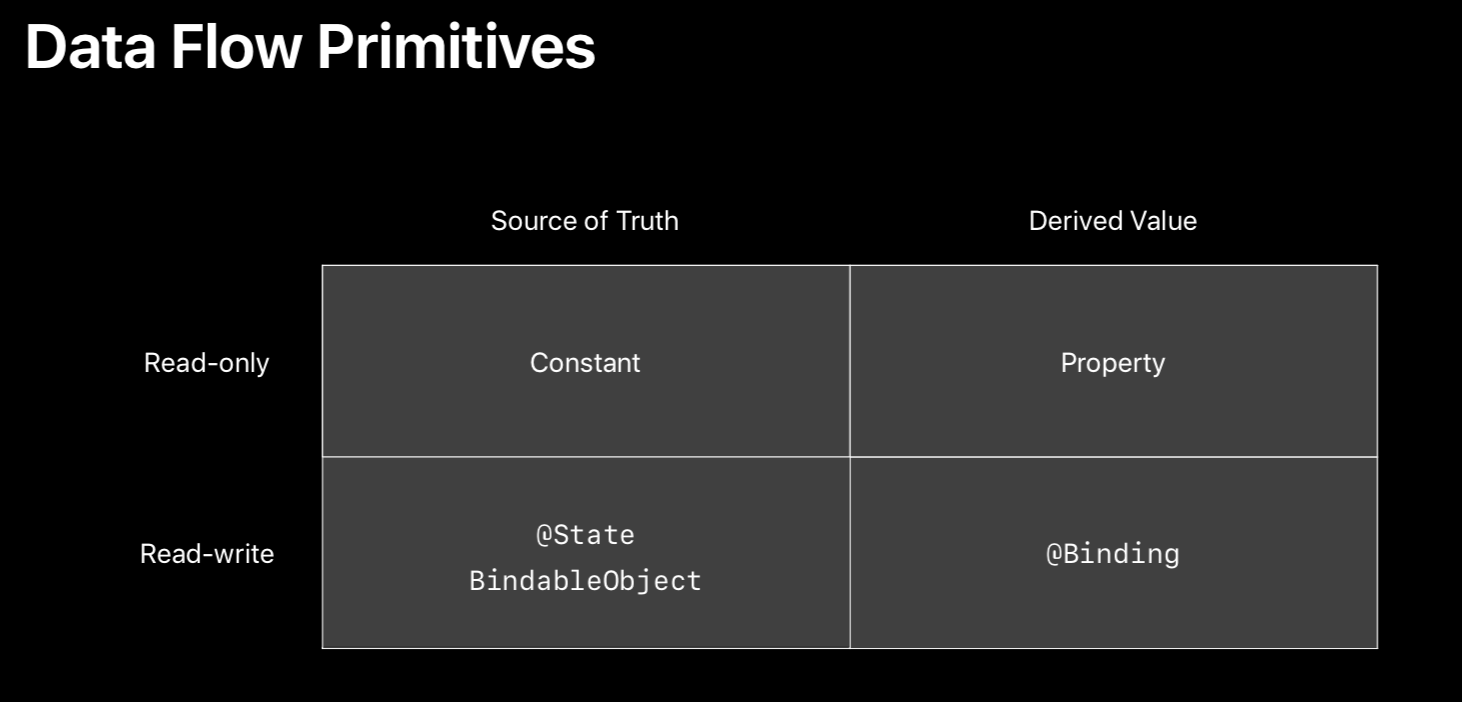
\includegraphics[width=1\textwidth]{images/DataFlowPrimitives.png}
\centering
\caption{\textit{Различити омотачи података}}
\label{slika:data_flow_primitives}
\end{figure}

% Dodati kod koji bolje objasnjava omotace podataka
\begin{lstlisting}[caption=\textit{{Омотачи података - State}}, label={lst:Омотачи података - State}, language=Swift, frame=single]
    struct Recept: View {
        var recept: ReceptPodatak
        @State private var daLiJeOmiljen: Bool = false
        
        var body: some View {
            VStack {
                Text(recept.ime)
                // 'OmiljenRecept' je pogled koji sadrzi zvezdicu koja oznacava da li je recept medju omiljenima (puna zvezdica - jeste, prazna - nije) 
                // Prosledjivanjem promenljive 'daLiJeOmiljen' uz prefiks '$' omogucava se promena promenljive 'daLiJeOmiljen' u pogledu 'OmiljenRecept'
                OmiljenRecept(daLiJe: $daLiJeOmiljen)
            }
        }
    }
\end{lstlisting}

\begin{lstlisting}[caption=\textit{{Омотачи података - Binding}}, label={lst:Омотачи података - Binding}, language=Swift, frame=single]
    struct Recept: View {
    // Promenljiva 'isPlaying' je definisana u jednom pogledu, a moze se menjati u drugom
    var recept: ReceptPodatak
    @Binding var daLiJeOmiljen: Bool

    var body: some View {
        Button(action: {
            // Akcija dugmeta koja menja promenljivu 'daLiJeOmiljen'
            self.daLiJeOmiljen.toggle()
        }) {
            // Provera promenljive 'daLiJeOmiljen' i prikaz odgovarajuce slike
            Image(systemName: daLiJeOmiljen ? "star.fill" : "star.empty")
        }
    }
}
\end{lstlisting}

\begin{lstlisting}[caption=\textit{{Омотачи података - Environment}}, label={lst:Омотачи података - Environment}, language=Swift, frame=single]
    struct Kulinarstvo_widgetEntryView : View {
    var entry: Provider.Entry
    
    // Citamo podatke za 'widgetFamily' iz okruzenja aplikacije (eng. Environment) i smestamo ih u promenljivu 'widgetFamily'
    @Environment(\.widgetFamily) var widgetFamily
    
    @ViewBuilder
    var body: some View {
        // U zavisnosti od promenljive 'widgetFamily' prikazujemo odgovarajuci widget
        switch widgetFamily {
        case .systemSmall:
            RecipeView(recipe: entry.recipe)
                .widgetURL(entry.recipe.url)
        case .systemMedium:
            RecipeMediumView(recipe: entry.recipe, ingredients: entry.recipe.ingredients.count > 3 ? Array(entry.recipe.ingredients.dropLast(entry.recipe.ingredients.count - 3)) : entry.recipe.ingredients)
        default:
            Text("")
        }
    }
}
\end{lstlisting}

\subsection{Разлика SwiftUI и UIKit}
\label{subsec:Разлика SwiftUI и UIKit}

\indent \textit{UIKit} и \textit{SwiftUI} су радна окружења развијена од стране \textit{Apple}-а, а која помажу приликом израде корисничког интерфејса апликације. Генерално, највећа разлика између ова два радна окружења је у начину размишљања, како доћи до решења и како то решење касније имплементирати. Ову разлику ће најбоље бити показана на једном конкретном примеру; Форма за пријављивање на одређени сајт, креирање вертикалног скупа елемената, хоризонтално и вертикално центрираних у том скупу, док се скуп састоји од два текстуална поља(корисничко име и лозинка) и дугмета(са акцијом провере података).
\\
\indent Са \textit{UIKit}-ом мора се водити рачуна о свим ситним детаљима као што су: креирање вертикалног скупа елемената, његово додавање у главни поглед, креирање текстуалног поља, додавање текстуалног поља у скуп елемената, додавање аутоматског ограничења распореда како би се центрирало текстуално поље, понављање поступка за друго текстуално поље и поновно понављање поступка за дугме. 
\\ % можда кораке прабацити у листу, због прегледности
\indent За разлику од тога, као што је напоменуто, \textit{SwiftUI} се базира на декларативном начину програмирања, и овде је довољно да навести груписање два текстуална поља и дугмета у вертиклани скуп елемената и у ком погледу ће се приказати. Све ситне детаље ће радно окружење одрадити уместо нас онако како је то уобичајено дефинисано. Наравно не мора се придржавати свих детаља које окружење одради, већ се могу по потреби променити.
\\
\indent Креирање корисничког интерфејса у \textit{UIKit}-у коришћењем само \textit{Swift} кода је веома компликовано, и за веће пројекте готово немогуће, јер се мора водити рачуна о сваком детаљу. Најчешћи начин израде корисничког интерфејса је коришћењем \textit{Storyboards-а} i \textit{Interface Builder-а}, помоћу којих програмер креира кориснички интерфејс превлачењем, спустањем и конфигурацијом елемената. У \textit{SwiftUI}-у се кориснички интерфејс изграђује помоћу \textit{Swift} кода. Једноставно се изјасни шта ће бити креирано и радно окружење то уради. Да би процес креирања био бржи и приступачнији, од верзије \textit{Xcode}-а 11, која је изашла у исто време када је представљен \textit{SwiftUI}, постоји могућност прегледа уживо сваког појединачног погледа који је креиран или скупа више погледа одједном. О овоме ће бити више речи у поглављу \ref{subsec:Xcode - преглед уживо} - \nameref{subsec:Xcode - преглед уживо}.
\\
\indent Уколико се сагледају архитектуре образаца, може се приметити да се \textit{UIKit} првенствено базира на \textit{MVC}\footnote{Архитектурни образац Модел-Поглед-Контролер (енг. Model-View-Controller) који се заснива на подели на три целине, модел - структура података, поглед - приказ података у корисничком окружењу, контролор - управљање моделом} обрасцу, док за разлику од њега, \textit{SwiftUI} користи \textit{MVVM}\footnote{Архитектурни образац Модел-Поглед-Модел погледа (енг. Model-View-ViewModel) који се заснива на подели на три целине, модел - структура података, поглед - приказ података у корисничком окружењу, модел погледа - стање података у моделу} образац. За заинтересоване читаоце, постоји могућност комбиновања два радна окружења и коришћење \textit{SwiftUI}-а унутар \textit{UIKit} кода, или обратно, али ово се оставља читаоцима да сами истраже како се то може постићи.

\subsection{Xcode - преглед уживо}
\label{subsec:Xcode - преглед уживо}

\indent Са представљањем \textit{SwiftUI}-a, \textit{Apple} је представио и нову верзију њиховог ИРО-а, \textit{Xcode11}, у коме је додато својство рада у новом радном окружењу као и могућност прегледа уживо сваког погледа. Предност оваквог начина писања кода је пре свега у могућности брзог прегледа измена и то без поновног обнављања (енг. rebuilding) апликације, поготово уколико се ради на додавању или измени погледа који се налази дубоко у навигацији апликације и за који је потребно више кликова и/или превлачења да би се до њега дошло. 
\\
\indent Преглед уживо помаже да се и у \textit{SwiftUI}-у користи метод превлачења и пуштања за креирање корисничког интерфејса, који се разликује од претходног који је коришћен унутар \textit{Storyboard}-а, јер сваки елемент се превлачи у део где се пише код и када се испусти тај елемент постаје део кода. 
% Слика превлачења и пуштања за SwiftUI 
Да би се омогућило коришћење приказа уживо, инстанца жељеног погледа се смешта унутар тела структуре која имплементира протокол \textit{PreviewProvider}, а која служи за живи приказ погледа или групе погледа. Пример употребе структуре која имплементира протокол \textit{PreviewProvider} може се видети у делу \ref{lst:Xcode - преглед уживо} - \nameref{lst:Xcode - преглед уживо}.

\begin{lstlisting}[caption=\textit{{Xcode - преглед уживо}}, label={lst:Xcode - преглед уживо}, language=Swift, frame=single]
    
    struct PlaceholderView : View {
        var body : some View {
            Kulinarstvo_widgetEntryView(entry: SimpleEntry(date: Date(), configuration: ConfigurationIntent(), recipe: RecipeModel.testData[0]))
        }
    }
    
    // Struktura u kojoj se konfigurise prikaz uzivo
    struct Kulinarstvo_widget_Previews: PreviewProvider {
        static var previews: some View {
            // Grupisanje vise pogleda
            Group {
                // Prikaz malog widget-a sa prvim elementom iz liste
                Kulinarstvo_widgetEntryView(entry: SimpleEntry(date: Date(), configuration: ConfigurationIntent(), recipe: RecipeModel.testData[0]))
                    .previewContext(WidgetPreviewContext(family: .systemSmall))
                
                // Prikaz srednjeg widget-a sa skrivenim sadrzajem
                PlaceholderView()
                    .previewContext(WidgetPreviewContext(family: .systemMedium))
                    .redacted(reason: .placeholder)
            }
        }
    }    
\end{lstlisting}

\indent Након сваке измене која се направи у коду који је везан за поглед(е) који се налази у прегледу уживо, \textit{Xcode} ће изнова направити нову верзију и покренути је у прозору за преглед уживо. Као што је виђено у примеру кода изнад, преглед уживо не мора приказивати само један поглед, већ се могу груписати различити погледи и све бити приказати одједном. Предност оваквог приступа је могућност истовременог прегледа старог и новог изгледа погледа, више величина \textit{widget}-а, истих погледа са светлом и тамном бојом позадине, погледа на различитим језицима...

% Слика преглед уживо

\indent За оне који желе да истраже више о овој теми, препорука је да одгледају два одлична клипа са \textit{Apple}-ове конференције за програмере из 2019. и 2020. године респективно. Клипови су: \href{https://developer.apple.com/videos/play/wwdc2019/233/}{\textit{'Mastering Xcode Previews'}} и \href{https://developer.apple.com/videos/play/wwdc2020/10149/}{\textit{'Structure your app for SwiftUI previews'}}.

\chapter{Улога и развој Widget-a}

\indent \textit{Widget}, као део мобилне апликациjе, се налази на почетном екрану уређаjа (телефона или таблета) и кориснику приказуjе одабране важне информациjе из те апликациjе. За разлику од \textit{widget}-а у оперативном систему \textit{Android}, коjи су присутни више од десет година, \textit{widgeti} на Apple платформама су уведени 2020. године, тако да jе и сама технологиjа коjа подржава њихово креирање и даље у активном развоjу.

\section{Основно}

\indent \textit{Widgeti} на уређајима са \textit{Apple} платформом узимају један од кључних делова апликације за коју је развијени и приказују га крајњим корисницима тамо где ће га најлакше уочити, на \textit{iPhone}-у и \textit{iPad}-у се може налазити на почетном екрану или у делу \textit{Today View}-а, док се на \textit{Mac} уређајима налазе у центру за нотификације. Величина \textit{widget}-а није флексибилна као на \textit{Android} уређајима, па тако постоји могућност креирања малих (величина 2x2 места на почетном екрану \textit{iPhone}-а), средњих (2x4), великих (4x4) и од верзије \textit{iPadOS15} екстра великих (4x8), само за \textit{iPad} уређаје, \textit{widget}-а. 
\\
\indent Скуп свих тренутно доступних \textit{widget}-а на уређају налази се у галерији \textit{widget}-а (енг. widget gallery), која помаже корисницима приликом одабира конкретне величине и типа \textit{widget}-а (Једна апликација може испоручити више типова \textit{widget}-а исте величине). Унутар галерије такође постоји опција за измену \textit{widget}-а у којој корисници могу да контролишу и мењају своје \textit{widget}-е и тиме их што више прилагоде себи, али само уколико је у току конструисања \textit{widget}-а од стране програмера то омогућено. Више речи о овоме биће у делу \ref{sec:Развој Widget-a} - \nameref{sec:Развој Widget-a}.
\\
\indent На оперативним системима \textit{iOS} и \textit{iPadOS}, галерија има могућност додавања паметних гомила (енг. smart stack), које могу садржати до 10 различитих \textit{widget}-а исте величине. Паметна гомила приказује само један од \textit{widget}-а који се налазе у њој. Корисник може сам да мења који ће \textit{widget} бити приказан једноставним померањем (енг. scrolling). Временом, паметна гомила може научити који \textit{widget} корисник ставља на почетак гомиле у току дана (или недеље) и сама мењати примарне \textit{widget}-е у одређеном тренутку (на пример, након гашења аларма прво се приказује \textit{widget} са временском прогнозом, па најновије вести, стање у саобраћају...)
\\
\indent \textit{Siri}\footnote{Интелигентни лични асистент на уређајима са \textit{Apple} платформом} може и сама додати \textit{widget}-е у паметну гомилу, уколико претпостави да постоји неки \textit{widget} који би кориснику био користан. Након тога, корисник сам одлучује да ли жели да новододати \textit{widget} остане у паметној гомили или не.

\subsection{WidgetKit}
\indent \textit{WidgetKit} је радно окружење, које уз \textit{widget API} из  \textit{SwiftUI}-а служи за израду \textit{widget}-а, од његовог изгледа преко временског ажурирања па све до омогућавања конфигурације \textit{widget}-а од стране крајњих корисника и управљања паметном гомилом приликом ротације \textit{widget}-а од стране самог система. Још једна могућност коју ово радно окружење пружа је повезивање апликације и самог \textit{widget}-а, што омогућава кориснику да отвори апликацију притиском на \textit{widget} и аутоматски оде на одговарајући поглед из \textit{widget}-а када жели да види детаљније податке. Пажња код ових ствари је да \textit{widget} не би смео да служи само као пречица за покретање апликације, више о томе биће објашњено у делу \ref{sec:Дизајн Widget-a} - \nameref{sec:Дизајн Widget-a}.

\section{Развој Widget-a}
\label{sec:Развој Widget-a}
\indent \textit{Widget} је ништа друго до заправо само један \textit{SwiftUI} поглед. \textit{Widgeti} су тренутно једини део оперативних система \textit{Apple}-а који у потпуности морају бити написани коришћењем радног оквира \textit{SwiftUI}. \textit{Apple} је отпочетка развоја \textit{widget}-а имао на уму овакву идеју, због начина приказивања података, повременог ажурирања података и немогућности корисничке интеракције са самим \textit{widget}-има (осим једноставног клика којим се отвара одређени део аплиакције).

\subsection{Додавање widget додатка апликацији}
\indent Шаблон за \textit{widget} додатак креира основне ставке потребне за његову израду. Унутар овог додатка корисник креира све потребне \textit{widget}-е за апликацију, независно од њиховог броја и величине. У посебним ситуацијама различити \textit{widgeti} могу бити одвојени у посебним додатцима, ово се најчешће односи када један тип \textit{widget}-а захтева одређене дозволе од стране корисника, док за други тип оне нису потребне (на пример, приступ тренутној локацији корисника).

\indent Кораци за креирање \textit{widget} додатка:
\begin{enumerate}
    \item Отворити пројекат у \textit{Xcode}-у и изабрати \textit{File -> New -> Target}
    % slika
    \item Из групе \textit{Application Extension}, изабрати \textit{Widget Extension} и кликнути \textit{Next}
    % slika
    \item Унети име додатка
    % slika
    \item Уколико ће \textit{widget} подржавати конфигурацију од стране корисника, штиклирати поље \textit{Include Configuration Intent}
    % slika
    \item Кликнути на \textit{Finish}
    % slika
\end{enumerate}

\subsection{Додавање детаља конфигурације}
\indent Као што је већ напоменуто, шаблон \textit{widget} додатка пружа иницијалну имплементацију \textit{widget}-а која имплементира \textit{Widget} протокол. Два могућа начина конфигурације \textit{widget}-а су статичка (енг. StaticConfiguration) и конфигурација са сврхом (енг. IntentConfiguration).
\indent Статичка конфигурација се користи за \textit{widget}-е који немају параметре који могу бити конфигурисани од стране корисника (на пример, системска апликација \textit{Screen time} која води статистику о времену проведеном на одговарајућем уређају).
\indent Конфигурација са сврхом се користи за \textit{widget}-е чији одређени параметри могу бити конфигурисани од стране корисника (на пример, системаска аплиакција за временску прогнозу где корисник може наместити одређени град за који жели да добија податке). Ова конфигурација ће бити укључена и конфигурациони фајл ће бити додат уколико је корисник приликом додавања \textit{widget} додатка, штиклирао поље \textit{Include Configuration Intent}.
\\
\indent Да би програмер спровео почетну конфигурацију \textit{widget}-а потребно је да проследи следеће параметре:
\begin{itemize}
    \item Тип (енг. Kind), стринг који идентификује \textit{widget}, требао би да казује шта \textit{widget} представља
    \item Снабдевач (енг. Provider), објекат класе која имплементира протокол \textit{TimelineProvider} и кроз временску линију коју производи одређује у ком тренутку ће \textit{widget} бити поново изрендерован и нови подаци бити приказани. Више о овом протоколу и свеукупној причи о временој линији у делу \ref{subsec:Временска линија} - \nameref{subsec:Временска линија}
    \item Затворење садржаја (енг. Content Closure), затворење које садржи поглед \textit{SwiftUI} и које \textit{WidgetKit} позива када дође време за поновно рендеровање садржаја \textit{widget-а}
    \item Прилагођена сврха (енг. Custom Intent), фајл који дефинише параметре које корисник може мењати и прилагођавати себи, више о овоме у делу: \ref{subsec:Intent} - \nameref{subsec:Intent}
\end{itemize}
% Kod za pocetnu konfiguraciju widget-a, uz dodatne parametre, ime za prikaz, opis, velicine widget-a, boja pozadine widget-a

\subsection{Временска линија}
\label{subsec:Временска линија}
\indent Снабдевач временске линије генерише временску линију која се састоји од уноса (енг. entries), а сваки унос садржи датум и време када је потребно ажурирати садржај \textit{widget}-а. Када се датум и време из уноса подударе са реалним временом, \textit{WidgetKit} позива затворење садржаја које потом приказује ажуриране податке. 
\\
\indent Да би \textit{widget} био приказан у \textit{widget} галерији, \textit{WidgetKit} захтева од снабдевача, преглед снимка (енг. Preview snapshot). Дохватање прегледа снимка се разрешава провером променљиве \textit{isPreview} којом се проверава да ли снабдевач прегледа снимка шаље тренутни снимак за приказ у галерији или за приказ \textit{widget}-а на почетном екрану (или \textit{Today} погледу, или центру за обавештења). Када је параметар \textit{isPreview} тачан, \textit{widget} се приказује у галерији. Уколико за приказ \textit{widget}-а треба да буду приказани и одређени подаци, а подаци нису пристигли са серверске стране, постоје два решења. Можемо приказати подразумеване, унапред одређене податке, или можемо користити податке које чувају место правим подацима (енг. placeholder). 
% Слика са placeholder podacima i objasnjenje kroz komentare
\\
\indent Када пристигну подаци са сервера, снабдевач добија обавештење, сакупља реалне податке и приказује \textit{widget} са њима. Након што корисник дода \textit{widget} на почетни екран и буде приказан иницијални снимак изгледа \textit{widget-а}, \textit{WidgetKit} позива функцију \textit{getTimeline} из провајдера, чиме захтева временску линију.
% Primer sa ovom funkcijom iz koda

\subsection{\textit{Intent}}
\label{subsec:Intent}
\indent \textit{Widget}-i предтављају погледе који не интерагују са корисницима, односно не подржавају интерактивне елементе, као што су поглед \textit{scroll} и дугме \textit{switch}. Једна врста интеракције корисника са \textit{widget}-ом постиже се омогућавањем конфигурације \textit{widget}-а од стране корисника коришћењем конфигурације \textit{Intent}, у којој се наводе сви параметри које корисник може да промени (и дозвољене вредности за те параметре). 
\\
\indent Да би се додали параметри које корисник може да конфигурише, постоје предуслови који се морају испунити:
\begin{itemize}
    \item Додавање дефиниције \textit{intent}-а који дефинише конфигурабилне параметре 
    \item Коришћење протокола \textit{IntentTimelineProvider} уместо протокола \textit{TimelineProvider} као провајдера временске линије, да би конфигурација параметара од стране корисника била сачувана у уносима временске линије
    \item Уколико параметри зависе од динамичких података потребно је имплементирати екстензију \textit{intent}-а
\end{itemize}
% Слике додавања intent-a и његова конфигурација, примери кода и приказ конфигурације параметара у симулатору

\subsection{Везе унутар \textit{widget}-а}
\indent Једини начин директне комуникације између корисника и \textit{widget}-а остварена је везама (енг. links) унутар \textit{widget}-а. Када корисник кликне на \textit{widget} отвара се апликација којој тај \textit{widget} припада, и може се конфигурисати који део апликације ће бити приказан кориснику у зависности од елемента унутар \textit{widget}-а на који је кликнуо. Свим величинама \textit{widget}-а може бити додат модификатор \textit{widgetURL(\_:)}, којим се одређује у који део апликације ће корисник бити одведен када кликне на \textit{widget}.
\\
\indent За све величине \textit{widget}-а, осим малих, могу се користити и везе које су додате једном елементу унутар \textit{widget}-а и којим је одређено место у апликацији које ће бити отворено (на пример, један \textit{widget} средње величине који садржи листу са 3 рецепата, сваки елемент листе има везу која води ка детаљној страни о рецепту који тај елемент представља). Иако \textit{widget} користи везе унутар својих елемената, може користити и модигикатор \textit{widgetURL(\_:)} из претходног примера. Овај модификатор ће бити активиран уколико корисник кликне на елеменат у \textit{widget}-у који нема дефинисану везу. 
% Примери кода

\subsection{Више \textit{widget}-а у једном проширењу}
\indent Уколико желимо да користимо више различитих типова \textit{widget}-а у једном проширењу, то можемо лако урадити уз само пар измена главног дела проширења, означеног атрибутом \textit{@main}. Уместо протокола \textit{Widget} главна структура мора имплементирати протокол \textit{WidgetBundle}. Тело структуре сада имплементира протокол \textit{Widget} и додата му је анотација \textit{@WidgetBundleBuilder}. Приказ употребе више типова у једном проширењу може се видети у примеру \ref{lst:Више widget-а у једном проширењу} - \nameref{lst:Више widget-а у једном проширењу}.

\begin{lstlisting}[caption=\textit{{Више widget-а у једном проширењу}}, label={lst:Више widget-а у једном проширењу}, language=Swift, frame=single]
    @main
    // Umesto protokola 'Widget', koristimo 'WidgetBundle'
    struct ReceptiWidgets: WidgetBundle {
        // Definisemo atribut '@WidgetBundlerBuilder'
        @WidgetBundleBuilder
        // Definisemo telo, koje ovog puta implementira protokol 'Widget'
        var body: some Widget {
            DetaljanPrikazReceptaWidget()
            ListaRecepataWidget()
            SpisakZaKupovinuWidget()
        }
    }
\end{lstlisting}

\section{Дизајн \textit{Widget}-a}
\label{sec:Дизајн Widget-a}

\indent Главна улога \textit{widget}-а је приказивање садржаја који кориснику пружа корисне информације без покретања апликације. Самим тим подаци морају бити тачни и релевантни за корисника, сам \textit{widget} би требао бити конфигурабилан како би кориснику допустио одређену врсту слободе прилком коришћења \textit{widget}-а и дизајниран тако да одговара апликацији којој припада.

\subsection{Фокус \textit{Widget}-a}
\indent  Подаци које приказује треба да буду минималистички, да одговарају величини \textit{widget}-а (већа величина треба да повлачи и већу количину података) и да буду временски и кориснички релевантни. Први корак у дизајну \textit{widget}-а је избор једног дела аплиакције који ће тај \textit{widget} представљaти. 
\\
\indent Свака величина \textit{widget}-а која је омогућена за додавање из галерије треба да садржи одређену количину информација која је пропорционална тој величини. Не сме се дозволити да више величина \textit{widget}-а приказују исте податке, али истовремено приликом додавања нових података се мора водити рачуна о почетној идеји, односно делу апликације које тај \textit{widget} треба да представља. Уколико не постоји довољна количина података за веће \textit{widget}-е (на пример, за \textit{widget} величине \textit{large}), одређене величине могу бити и искључене из понуде кориснику.
\\
\indent \textit{Widget} не би смео да служи само као пречица за покретање аплиакције. Корисници очекује од сваког \textit{widget}-а да им покаже корисне информације, у супротном неће наићи на добар одзив и истовремено може бити штетно самој апликацији (мањи број корисника, лошија оцена у продавници).

\subsection{Ажурни подаци}
\indent Да би \textit{widgeti} могли да пружају корисне и прецизне информације у скоро сваком тренутку, морају повремено бити ажурирани. \textit{Widgeti} не подржавају ажурирање у реалном времену, а и сам систем може ограничити ажурирање \textit{widget}-а у завиности од корисничког понашања и интеракције са њим, па се морамо потрудити да нађемо начин на који ће подаци у нашем \textit{widget}-у увек бити релевантни. 
\\
\indent Потребно је пронаћи оптимално време за ажурирање података у \textit{widget}-у, узимајући у обзир колико се сами подаци често мењају и колико често корисницима може бити корисно да виде те податке. Уколико након публикације \textit{widget}-а уочимо да су корисницима чешће или ређе потребни новији подаци, можемо променити време између два ажурирања и тиме побољшати корисничко искуство. Још једна корисна ствар код информација које су временски зависне (на пример, тренутно стање неког индекса или акције на берзи), можемо у \textit{widget}-у додати и поље које ће представљати датум  и време када су подаци последњи пут ажурирани. Иако не можемо да приказујемо податке у реалном времену, за неке податке можемо искористити помоћ система за одређивање датума и времена, па тако уколико би имали \textit{widget} који приказује време у које ће се огласити аларм, истовремено можемо имати и ажуран податак о томе колико је времена остало до оглашавања аларма.  

\subsection{Конфигурабилност и интеракција}
\indent У већини случајева \textit{widget} треба да омогући кориснику конфигурабилност како би пружио корисне информације (на пример, књига коју корисник тренутно чита и његов прогрес у апликацији \textit{Apple Books}), док поједине апликације могу то да изоставе (на пример, најновије вести). Уколико је \textit{widget} конфигурабилан, потребно је да подешавања буду што једноставнија и да се не траже превише информација од корисника. Кориснички интерфејс за измену \textit{widget}-а је унапред одређен и исти за све, као што је показано у делу \ref{subsec:Intent} - \nameref{subsec:Intent}.
\\
\indent Када корисник кликне на \textit{widget} или део унутар њега, за веће величине, очекује да буде одведен на жељену страницу, да не мора да претражује и даље апликацију (на пример, када кликне на одређени рецепт у \textit{widget}-у, желеће да му се отвори страница са детаљним приказом тог рецепта, а не почетна страна). Истовремено, треба се избећи превише веза на малом простору, где се лако може десити да због густине распореда, корисник кликне грешком на један елемент, а желео је да притисне сасвим други.

\subsection{Дизајн прилагођен свима}
\indent \textit{Widgeti} треба да имају јарке боје како би се истицали на екрану, али истовремено и јасно видљив текст како би корисник могао да види све потребне информације "бацањем погледа" након откључавања или непосредно пре закључавања уређаја. \textit{Widget} треба прилагодити апликацији коју представља (боје, фонт текста, јединствени елементи...), док истовремено не треба претерати са обележјима.  
\\
\indent Количина информација коју ће бити приказана у \textit{widget}-у мора бити оптимална. Уколико се прикаже премало информација \textit{widget} неће имати превелики значај за кориснике, док превише информација на мало простора отежава читање и разумевање података.
\\
\indent Једна од битнијих ствари која се не сме заборавити у данашње време је дизајн \textit{widget}-а за обе врсте боја системске позадине (светле и тамне). Дизајн оба \textit{widget}-а се не сме разликовати од системске боје позадине јер ниједан корисник не жели видети таман текст на светлој боји позадине уколико је изабрао тамну системску боју позадине. Приликом израде обе врсте дизјна може помоћи \textit{Xcode preview} који омогућава истовремено сагледавање оба дизајна, упоређивање и исправљање евентуалних недостатака.
\\
\indent \textit{Apple} саветује да се никад не користи фонт текста мањи од 11 поена\footnote{\textit{Apple}-ов израз за "број који треба уписати у поље", универзална мера у дизајну на \textit{Apple} платформама}. Коришћење мањег фонта би корисницима знатно отежало употребу \textit{widget}-а. Поред овога, увек се требају користити званични елементи за приказ текста, како би се омогућила скалабилност као и системско читање текста. 
\\
\indent Пажњу треба обратити на дизајн прегледа \textit{widget}-а унутар галерије, за све типове и величине који \textit{widget} подржава, као и приказ чувара места уместо реалних података уколико они нису пристигли на време са сервера и непостоје подразумевани подаци. Уколико се исти елементи налазе у апликацији и истовремено на \textit{widget}-у потребно је да имају исту функционалност јер би у супротном корисници били збуњени. 
\\
\indent Потребно је искористити могућност приказа описа \textit{widget}-а у галерији и саставити кратак и јасан опис функционалности \textit{widget}-а. Груписање свих величина једног типа \textit{widget}-а са јединственим описом је погодно корисницима апликације, пре свега због једноставности разумевања коришћења \textit{widget}-а.
\\
\indent Скалабилност елемената унутар \textit{widget}-а је веома важна јер систем аутоматски прилагођава величину \textit{widget}-а величини екрана уређаја, зато је потребно обратити пажњу приликом додавања елемената. Најбоље је користити проверене елементе који пружају флексибилност, у овом случају било који основни \textit{SwiftUI} елемент или њихова комбинација.

\chapter{Опис апликације}

\chapter{Закључак}

\literatura

\end{document}
